\documentclass{IFES-beamer}

% --------------------------------------------------- %
%           Información de la Presentación	          %
% --------------------------------------------------- %
\title[Pruebas con LaTeX Beamer Tikz]{Pruebas con LaTeX Beamer Tikz}
\subtitle{Actividad de Ejemplos y Ejercicios}
\author{Dylan Rodas}
\institute[UNIS]{
  Universidad del Istmo de Guatemala\\
  Facultad de Ingeniería
}
\date{30 de Noviembre, 2018}
\logo{

\includegraphics[scale=0.5]{Resources/Logo_UNIS.png}
}
\subject{Prácticas de Trabajo e Investigación 4}

% --------------------------------------------------- %
%             Título + Tabla de Contenidos            %
% --------------------------------------------------- %

\begin{document}

\begin{frame}
  \titlepage
\end{frame}

\begin{frame}{Contenido}
  \tableofcontents
\end{frame}

% --------------------------------------------------- %
%                      Presentación                   %
% --------------------------------------------------- %

\section{Dibujando con Tikz}
\begin{frame}{Dibujando una Línea}
\centering
\begin{tikzpicture}
\draw (0,0) -- (1,1); % una línea
\end{tikzpicture}
\end{frame}

\section{Coordenadas}
\begin{frame}{Dibujando una Coordenada}
\centering

\begin{tikzpicture}
\draw[help lines] (0,0) grid (3,3);
\end{tikzpicture}
\end{frame}

\section{Tipos de Líneas}
\begin{frame}{Dibujando los Tipos de Líneas}
\centering
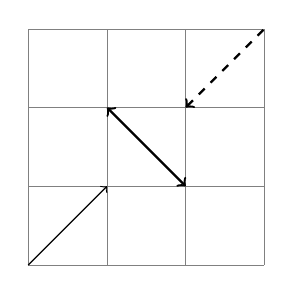
\begin{tikzpicture}
\draw[help lines] (0,0) grid (3,3);
\draw[->] (0,0) -- (1,1);
\draw[<->, thick] (2,1) -- (1,2);
\draw[<-, thick, dashed] (2,2)--(3,3);
\end{tikzpicture}
\end{frame}

\section{Trayectorias}
\begin{frame}{Dibujando Trayectorias}
\centering
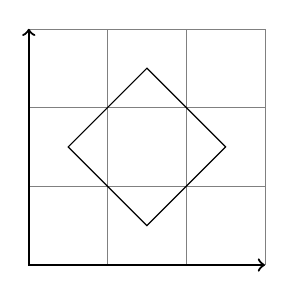
\begin{tikzpicture}
\draw[help lines] (0,0) grid (3,3);
% ejes:
\draw[<->, thick] (0,3)--(0,0)--(3,0);
% diamante:
\draw (1.5,0.5) -- (2.5,1.5) --
(1.5,2.5) -- (0.5,1.5) --
cycle; % cierre de trayectoria
\end{tikzpicture}
\end{frame}

\section{Colores}
\begin{frame}{Coloreando la Trayectoria}
\centering
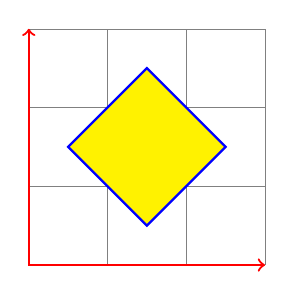
\begin{tikzpicture}
\draw[help lines] (0,0) grid (3,3);
% ejes
\draw[<->, thick, red]
(0,3)--(0,0)--(3,0);
% diamante
\draw[thick, blue, fill=yellow]
(1.5,0.5) -- (2.5,1.5) --
(1.5,2.5) -- (0.5,1.5) --
cycle;
\end{tikzpicture}
\end{frame}

\section{Figuras}
\begin{frame}{Figuras Simples}
\centering
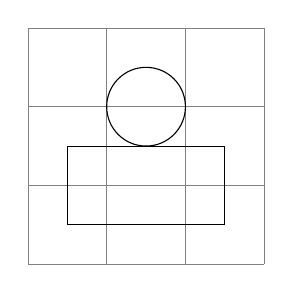
\begin{tikzpicture}
\draw[help lines] (0,0) grid (3,3);
\draw (1.5,2.0) circle (0.5);
\draw (0.5,0.5) rectangle (2.5,1.5);
\end{tikzpicture}
\end{frame}

\section{Nodos y Etiquetas}
\begin{frame}{Colocando Nodos y Etiquetas}
\centering
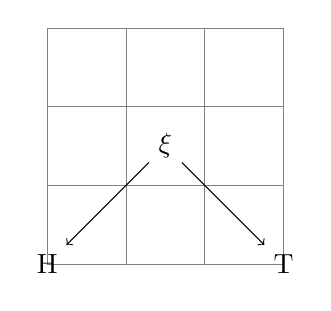
\begin{tikzpicture}
\draw[help lines] (0,0) grid (3,3);
\node (h) at (0,0) {H};
\node (x) at (1.5,1.5) {$\xi$};
\node (t) at (3,0) {T};
\draw[->] (x) -- (h);
\draw[->] (x) -- (t);
\end{tikzpicture}
\end{frame}

\section{Funciones}
\begin{frame}{Trazando una Función}
\centering
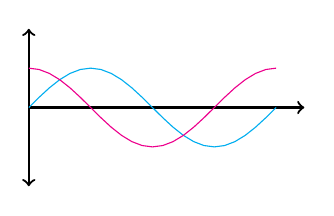
\begin{tikzpicture}[scale=0.5]
% eje y
\draw[<->, thick] (0,2) -- (0,-2);
% eje x
\draw[ ->, thick] (0,0) -- (7, 0);
% curvas
\draw[cyan,domain=0:2*pi]
plot (\x, {sin(\x r)});
\draw[magenta,domain=0:2*pi]
plot (\x, {cos(\x r)});
\end{tikzpicture}
\end{frame}

\section{Ejercicio}
\begin{frame}{Dibujando el Ejercicio con Tikz}
\centering
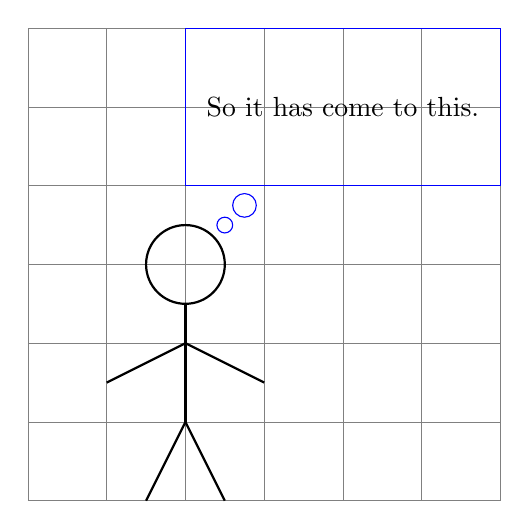
\begin{tikzpicture}
% Coordenadas
\draw[help lines] (0,0) grid (6,6);
% Cabeza y Cuerpo
\draw[thick] (2.0,3.0) circle (0.5);
\draw[thick] (2,2.5) -- (2,1);
\draw[thick] (2,2) -- (1,1.5);
\draw[thick] (2,2) -- (3,1.5);
\draw[thick] (2,1) -- (1.5,0);
\draw[thick] (2,1) -- (2.5,0);
% Pensamiento
\draw[blue] (2,4) rectangle (6,6);
\draw[blue] (2.5,3.5) circle (0.1);
\draw[blue] (2.75,3.75) circle (0.15);
\node (Texto) at (4,5) {So it has come to this.};
\end{tikzpicture}
\end{frame}

\end{document}